%-------------------------
%clang
%(c) H.Buchmann FHNW 2008
%export TEXINPUTS=.:${HOME}/fhnw/edu/:${HOME}/fhnw/edu/tinL/config/latex:${HOME}/fhnw/edu/config//:
%-------------------------
\documentclass{beamer}
\usepackage{beamer}
%---------------------
%local defines
%(c) H.Buchmann FHNW 2009
%$Id$
%---------------------
\newcommand{\target} {\beaglebone\xspace}
\newcommand{\targetS}{{\bf BBG}\xspace}
\newcommand{\host}   {{\em Host}\xspace}
\newcommand{\targetroot} {{\bf target-root}\xspace}
\newcommand{\kernel} {{\bf kernel}\xspace}
\renewcommand{\c}{{\bf C}\xspace}
\newcommand{\cpp}{{\bf C++}\xspace}
\newcommand{\posix}{{\bf POSIX}\xspace}

\input{/home/buchmann/latex/dirtree/dirtree.tex}

\usepackage[absolute]{textpos}
\setlength{\TPHorizModule}{1mm}
\setlength{\TPVertModule}{1mm}

\begin{document}

\title[clang]{clang:\\der andere Compiler}

\frame{\titlepage}

\begin{frame}{Ein anderer (als {\em gcc}):  {\em neuer} Compiler}{Warum}
 \begin{itemize}
  \item \cod{gcc} GNU Compiler Collection
  \begin{itemize}
   \item relativ alt
   \item etwas verrostet
   \item schwierig anzupassen
   \item GPL Lizenz f�r Firmen nicht immer optimal
  \end{itemize}
  \remark{GCC war (und ist) wichtig}
 \end{itemize}
\end{frame}

\begin{frame}{Andere Compiler}
 \begin{itemize}
  \item \url{http://en.wikipedia.org/wiki/List\_of\_compilers}
 \end{itemize}
 \remark{es gibt viele}
\end{frame}

\section{�bersicht}


\begin{frame}{Ein paar Begriffe}
  \begin{description}
   \item[HLL] {\bf H}igh {\bf L}evel programming {\em L}anguage
   \begin{itemize}
    \item C, C++, Fortran, Java 
   \end{itemize}
   \item[Target] Rechnerarchitektur
   \begin{itemize}
    \item ARM, x86, x86\_64 
   \end{itemize}
   \item[TASM] {\bf T}arget {\bf A}s{\bf S}e{\bf M}bler 
   \begin{itemize}
    \item Maschineninstruktionen f�r ein {\em Target}
   \end{itemize}
   \item[ObjectFile] Der Maschinencode bin�r verpackt
   \begin{itemize}
    \item Ein Format ELF: {\bf E}xecutable and {\bf L}inkable {\bf F}ormat
   \end{itemize}
  \end{description}
\end{frame}

\begin{frame}{Module$\to$Projekt}{Viele Files bilden ein Projekt}
 \begin{center}
 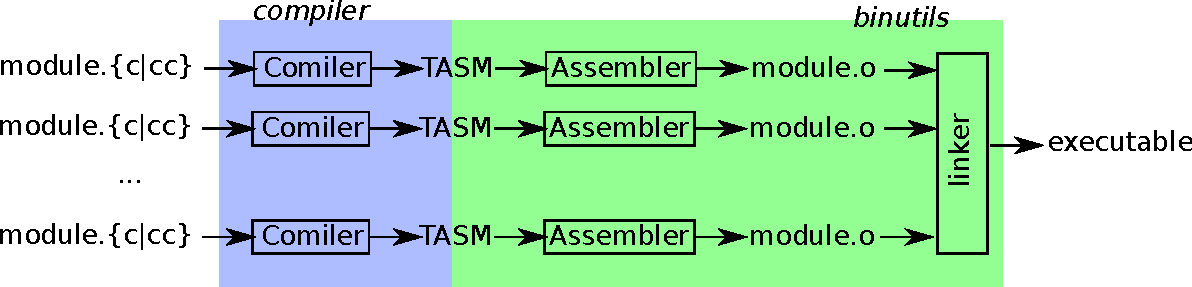
\includegraphics[width=11cm]{toolchain.pdf}
 \end{center}
 \begin{itemize}
  \item \cod{gcc -v hello-world.c -o hello-world} 
 \end{itemize}
\end{frame}

\begin{frame}{Die {\em CompileChain}}
 
\includegraphics[width=11cm]{compile-chain.pdf}
 \begin{itemize}
  \item \cod{gcc -c hello-world.c -o hello-world.o} 
  \begin{itemize}
   \item der normale Fall
  \end{itemize}
  \item \cod{gcc {\bf -v} -c hello-world.c -o hello-world.o} 
  \begin{itemize}
   \item {\bf -v} was passiert genau
  \end{itemize}
 \end{itemize}
 \begin{remarks}
  \item Input: 1 HLL File, Output 1 ObjectFile
  \item Der Assembler wird automatisch aufregrufen
 \end{remarks}
 \hfill{$\to$ unser Fokus: der Compiler}
\end{frame}

\section{Der Compiler}
\begin{frame}{Der Compiler}
 \fig{compiler.pdf}{1}{0}
 \begin{description}[Anforderung]
  \item[Input] {\em HLL} (praktisch) unabh�ngig vom {\em Target}
  \item[Output] {\em TASM} praktisch unabh�ngig von der {\em HLL}
  \item[Anforderung] {\em HLL} und {\em TASM} sollen {\Huge semantisch} gleich sein
 \end{description}
 \begin{remarks}
  \item {\em TASM} kann schon in bin�rer Form vorliegen
 \end{remarks}
\end{frame}

\begin{frame}{Aufbau}{gilt f�r fast alle Compiler}
 \begin{columns}
  \begin{column}{6.5cm}
    \fig{front-backend.pdf}{1}{0}
   \end{column}
   \begin{column}{5.5cm}
    \begin{description}
     \item[frontend] unabh�ngig vom {\em Target}
     \item[backend]  unabh�ngig von der  {\em HLL}
    \end{description}
   \end{column}
 \end{columns}
 \begin{itemize}
  \item {\color{red} Was liegt dazwischen ?}
 \end{itemize}
\end{frame}

\subsection{Intermediate Representation}

%\begin{frame}{IR: Intermediate Representation}{Universeller Assembler}
% \fig{intermediate-rep.pdf}{1}{0}
% \vspace{-1.5cm}
% \begin{itemize}
%  \item {\em HLL} $\to$ {\em IR} relativ einfach
%  \item {\em IR}  $\to$ {\em TASM} relativ einfach
%  \item {\color{red}Dazwischen} {\em HLL} {\bf und} {\em Target} unabh�ngige Operationen:
%  \begin{itemize}
%   \item Optimierung
%  \end{itemize}
%  komplex/kompliziert
% \end{itemize}
%\end{frame}

\begin{frame}{IR: Intermediate Representation}{Vorteil}
 \fig{hll-ir-tasm.pdf}{1}{0}
% \begin{description}
%  \item[HLL] viele einfache
%  \item[IR] nur einmal 
%  \item[TASM] viele einfache
% \end{description}
 \hfill{Was ist eine gute IR}
\end{frame}

\begin{frame}{IR}{Ein paar Beispiele}
\begin{description}
 \item[ByteCode] {\small\url{www.oracle.com/technetwork/java/index.html}}
 \begin{description}
  \item[HLL] Java, Scala
  \item[TASM] fast alle Platformen (Targets)
 \end{description}
 \item[GENERIC] {\small\url{https://gcc.gnu.org}}
 \begin{description}
  \item[HLL]  {\small\url{https://gcc.gnu.org/frontends.html}}
  \item[TASM] {\small\url{https://gcc.gnu.org/backends.html}}
 \end{description}
\end{description}
\end{frame}

\section{LLVM/clang}
\begin{frame}{IR}{LLVM \url{llvm.org}}
 \begin{description}
  \item[HLL]Ada, C, C++, D, Fortran,Objective-C \footnote{\url{en.wikipedia.org/wiki/LLVM}}
  \item[TASM] \cod{llvm-config --targets-built}
 \end{description}
\end{frame}

\newcommand{\enter}{$\backslash$\\}
\begin{frame}{�bersicht}
 \begin{itemize}
  \item wie \cod{gcc}
  \item Intermediate Representation
  \begin{itemize}
   \item {\em HLL}$\to${\em IR}
   \item {\em IR} $\to${\em TASM}
   \item {\em IR} Virtual Machine
  \end{itemize} 
 \end{itemize}
\end{frame}

\begin{frame}{\cod{gcc} like}{die gleichen Optionen}
 \begin{description}[direct verbose]
  \item[direct]\cod{clang hello-world.c -o hello-world}
  \item[direct verbose] \cod{clang -v hello-world.c -o hello-world}
  \item[compile-link] f�r Module
  \begin{description}
   \item[compile] \cod{clang -c hello-world.c\enter -o hello-world.o}
   \item[link] \cod{gcc hello-world.o \enter -o hello-world}
  \end{description}
  \item[TASM] Lesbare Maschineninstruktionen
  \begin{itemize}
   \item  \cod{clang -S hello-world.c -o hello-world.s}
  \end{itemize}
 \end{description}
\end{frame}

\begin{frame}{Intermediate Representation}
 \begin{block}{compile}
  \cod{clang -c -emit-llvm hello-world.c -o hello-world.bc}
 \end{block}
 \begin{block}{link}
  \cod{llvm-link hello-world.bc -o hello-world.llvm}
 \end{block}
 \begin{block}{interpret}
  \cod{lli c-hello-world.llvm}
 \end{block}
\end{frame}

\begin{frame}{Intermediate Representation}{Wie sieht er aus}
 \begin{description}
  \item[disassemble] \cod{llvm-dis  hello-world.bc -o -} 
  \begin{itemize}
   \item nach \cod{stdout}
  \end{itemize}
  \item[clang] \cod{clang -S -emit-llvm hello-world.c  \enter -o hello-world.llvm}
 \end{description}
\end{frame}

\begin{frame}{Warum \cod{llvm}/\cod{clang}}
 \begin{itemize}
  \item �bersichtliche Aufteilung {\em front-/backend} 
  \begin{itemize}
   \item Eigene {\em front-/backends} sind m�glich
   \remark{Auch mit \cod{gcc} m�glich aber viel un�bersichtlicher} 
  \end{itemize}
  \item Klar dokumentierte {\em Intermediate Representation}
  \item Modularer Aufbau der Software geschrieben in C++
  \item Grosse Firmen - Apple/Google - steht dahinter
 \end{itemize}
\end{frame}

\section{Aufgaben}
\begin{frame}{Aufgaben}
 \begin{description}
  \item[Installation] als source  oder als package
  \item[\raspberry]  \cod{clang} als Compiler
  \item[Vergleich] \cod{gcc} vs. \cod{clang}
  Beispiel \cod{prime-number.cc}
 \end{description}
\end{frame}

\end{document}
